
\documentclass[useAMS,usenatbib,article]{mn2e}

\usepackage{longtable}
\usepackage[]{graphicx}
\usepackage{amsmath}
\usepackage{natbib}
\bibliographystyle{mn2e}
%\usepackage{tabularx}
%\usepackage{bm}
%\usepackage{color}
%\usepackage{hyperref}

%% Sometimes a paper's abstract is too long to fit on the
%% title page in preprint2 mode. When that is the case,
%% use the longabstract style option.

%% \documentclass[preprint2,longabstract]{aastex}
\newcommand\aj{{AJ}}%
\newcommand\actaa{{Acta Astron.}}%
\newcommand\araa{{ARA\&A}}%
\newcommand\apj{{ApJ}}%
\newcommand\apjl{{ApJ}}%
\newcommand\apjs{{ApJS}}%
\newcommand\ao{{Appl.~Opt.}}%
\newcommand\apss{{Ap\&SS}}%
\newcommand\aap{{A\&A}}%
\newcommand\aapr{{A\&A~Rev.}}%
\newcommand\aaps{{A\&AS}}%
\newcommand\azh{{AZh}}%
\newcommand\baas{{BAAS}}%
\newcommand\caa{{Chinese Astron. Astrophys.}}%
\newcommand\cjaa{{Chinese J. Astron. Astrophys.}}%
\newcommand\icarus{{Icarus}}%
\newcommand\jcap{{J. Cosmology Astropart. Phys.}}%
\newcommand\jrasc{{JRASC}}%
\newcommand\memras{{MmRAS}}%
\newcommand\mnras{{MNRAS}}%
\newcommand\na{{New A}}%
\newcommand\nar{{New A Rev.}}%
\newcommand\pra{{Phys.~Rev.~A}}%
\newcommand\prb{{Phys.~Rev.~B}}%
\newcommand\prc{{Phys.~Rev.~C}}%
\newcommand\prd{{Phys.~Rev.~D}}%
\newcommand\pre{{Phys.~Rev.~E}}%
\newcommand\prl{{Phys.~Rev.~Lett.}}%
\newcommand\pasa{{PASA}}%
\newcommand\pasp{{PASP}}%
\newcommand\pasj{{PASJ}}%
\newcommand\qjras{{QJRAS}}%
\newcommand\rmxaa{{Rev. Mexicana Astron. Astrofis.}}%
\newcommand\skytel{{S\&T}}%
\newcommand\solphys{{Sol.~Phys.}}%
\newcommand\sovast{{Soviet~Ast.}}%
\newcommand\ssr{{Space~Sci.~Rev.}}%
\newcommand\zap{{ZAp}}%
\newcommand\nat{{Nature}}%
\newcommand\iaucirc{{IAU~Circ.}}%
\newcommand\aplett{{Astrophys.~Lett.}}%
\newcommand\apspr{{Astrophys.~Space~Phys.~Res.}}%
\newcommand\bain{{Bull.~Astron.~Inst.~Netherlands}}%
\newcommand\fcp{{Fund.~Cosmic~Phys.}}%
\newcommand\gca{{Geochim.~Cosmochim.~Acta}}%
\newcommand\grl{{Geophys.~Res.~Lett.}}%
\newcommand\jcp{{J.~Chem.~Phys.}}%
\newcommand\jgr{{J.~Geophys.~Res.}}%
\newcommand\jqsrt{{J.~Quant.~Spec.~Radiat.~Transf.}}%
\newcommand\memsai{{Mem.~Soc.~Astron.~Italiana}}%
\newcommand\nphysa{{Nucl.~Phys.~A}}%
\newcommand\physrep{{Phys.~Rep.}}%
\newcommand\physscr{{Phys.~Scr}}%
\newcommand\planss{{Planet.~Space~Sci.}}%
\newcommand\procspie{{Proc.~SPIE}}%


%\newcommand{\vdag}{(v)^\dagger}
%\newcommand{\myemail}{gsavorgn@astro.swin.edu.au}
%\newcommand{\fitfigurewidth}{0.8\textwidth}


\title[Intermediate-scale discs]{Early-type galaxies with intermediate-scale discs and their supermassive black holes}

\author[G.~A.~D. Savorgnan \& A.~W. Graham]
{\parbox{\textwidth}{
Giulia~A.~D. Savorgnan$^{1}$\thanks{E-mail: \texttt{gsavorgn@astro.swin.edu.au}},
Alister W. Graham$^{1}$}\vspace{0.4cm}\\
\parbox{\textwidth}{
$^{1}$Centre for Astrophysics and Supercomputing, Swinburne University of Technology, Hawthorn, Victoria 3122, Australia.\\}}

\pagerange{\pageref{firstpage}--\pageref{lastpage}} \pubyear{2015}

\begin{document}

\maketitle

\label{firstpage}



\begin{abstract}
vjsfkajhda
\end{abstract}

\begin{keywords}
black hole physics -- galaxies: bulges -- galaxies: elliptical and lenticular, cD -- galaxies: evolution -- galaxies: structure
\end{keywords}

\section{Introduction}
\label{sec:int}
There are currently two well-known types of stellar discs in galaxies. 
The first are the large-scale discs (with sizes of a few kiloparsec) that dominate the light at large radii in spiral and lenticular galaxies; 
the second are the small (tens to a couple of hundred parsec) nuclear discs observed in both early- and late-type galaxies 
(e.g.~\citealt{scorzavandenbosch1998,rest2001,balcells2007,ledo2010}). 
The origin of the nuclear discs has been speculated to arise from the infall of small satellite galaxies or gas clouds.  
The origin, or at least the on-going feeding and growth, of the large-scale discs has been attributed to cold gas flows, 
gas rich mergers and halo accretion events (e.g.~\citealt{khochfarsilk2006,dekel2009nat,dekel2009apj,ceverino2010,ceverino2012,conselice2012}). 
A thorough review can be found in Combes (arXiv:1309.1603 and 1405.6405).
On the other hand, intermediate-sized discs have not received the same level of attention as their nuclear and large-scale homologues, 
and, in some cases, they have even been labelled as something ''unphysical''. 
Here we report on the photometric and kinematical signatures of these intermediate-sized stellar discs 
and the impact this has on the important (black hole mass)-to-(spheroid stellar mass) ratio, $M_{\rm BH}/M_{*,sph}$, 
which is used to constrain galaxy evolution models.

%A puzzling question, which has been unspoken for decades, is why are there not intermediate-sized discs: 
%why are there not accretion events which create discs larger than the typical nuclear discs but which are not large enough to dominate at large radii? 

\section{Rationale}
\label{sec:rat}
The majority of stellar discs have some level of inclination with respect to our line-of-sight, 
and this makes them appear elliptical (rather than round) when seen in projection on the sky. 
This can help one distinguish them from the more spherically-shaped spheroids. 
Identifying the extent of these discs with respect to their spheroid can however be subtle. 
Two-dimensional kinematic maps represent an important diagnostic tool for this purpose. 
Most early-type galaxies are classified as ``central fast rotators'' \citep{atlas3dIII-MNRAS}, 
that is, they are rapidly rotating within their half-light radius.  
However, more extended kinematic maps \citep{arnold2014} reveal that 
some of the central fast rotators continue to be fast rotating at large radii, 
whereas other central fast rotators become slow rotators in their outer regions.
On the one hand, a specific angular momentum profile that is rapidly increasing beyond $1-2$ half-light radii 
is a signature of a large-scale disc. 
On the other hand, a specific angular momentum profile that increases up to $1-2$ half-light radii and declines beyond that point 
indicates the presence of an intermediate-scale disc that no longer dominates at large radii. 
Unfortunately, such extended kinematic maps are not yet available for large numbers of galaxies in the local Universe. 
Nevertheless, the ellipticity profile of a galaxy's isophotes can help identify the extent of stellar discs in early-type galaxies.

The toy model shown in Figure \ref{fig:model} illustrates the typical ellipticity profile 
($\epsilon = 1 - b/a$, where $b/a$ is the ratio of minor-to-major axis length) of 
(i) a lenticular galaxy, comprised of a large-scale disc and a relatively smaller encased bulge, 
(ii) an elliptical galaxy with a nuclear stellar disc, 
and (iii) a galaxy composed of an intermediate-scale disc embedded in a relatively larger spheroid. 
%We refer to the last case as an ellicular galaxy. 
In general, stellar discs are intrinsically flat and circular; 
their ellipticity, dictated by their inclination to our line of sight, is fixed. 
Spheroids are often rounder than the observed projection on the sky of their associated discs, 
thus their average ellipticity is often lower than that of their disc. 
An ellipticity profile that increases with radius can be ascribed to an inclined disc that becomes progressively more important at large radii, 
whereas a radial decrease of ellipticity signifies the opposite case. 

\begin{figure}
\begin{center}
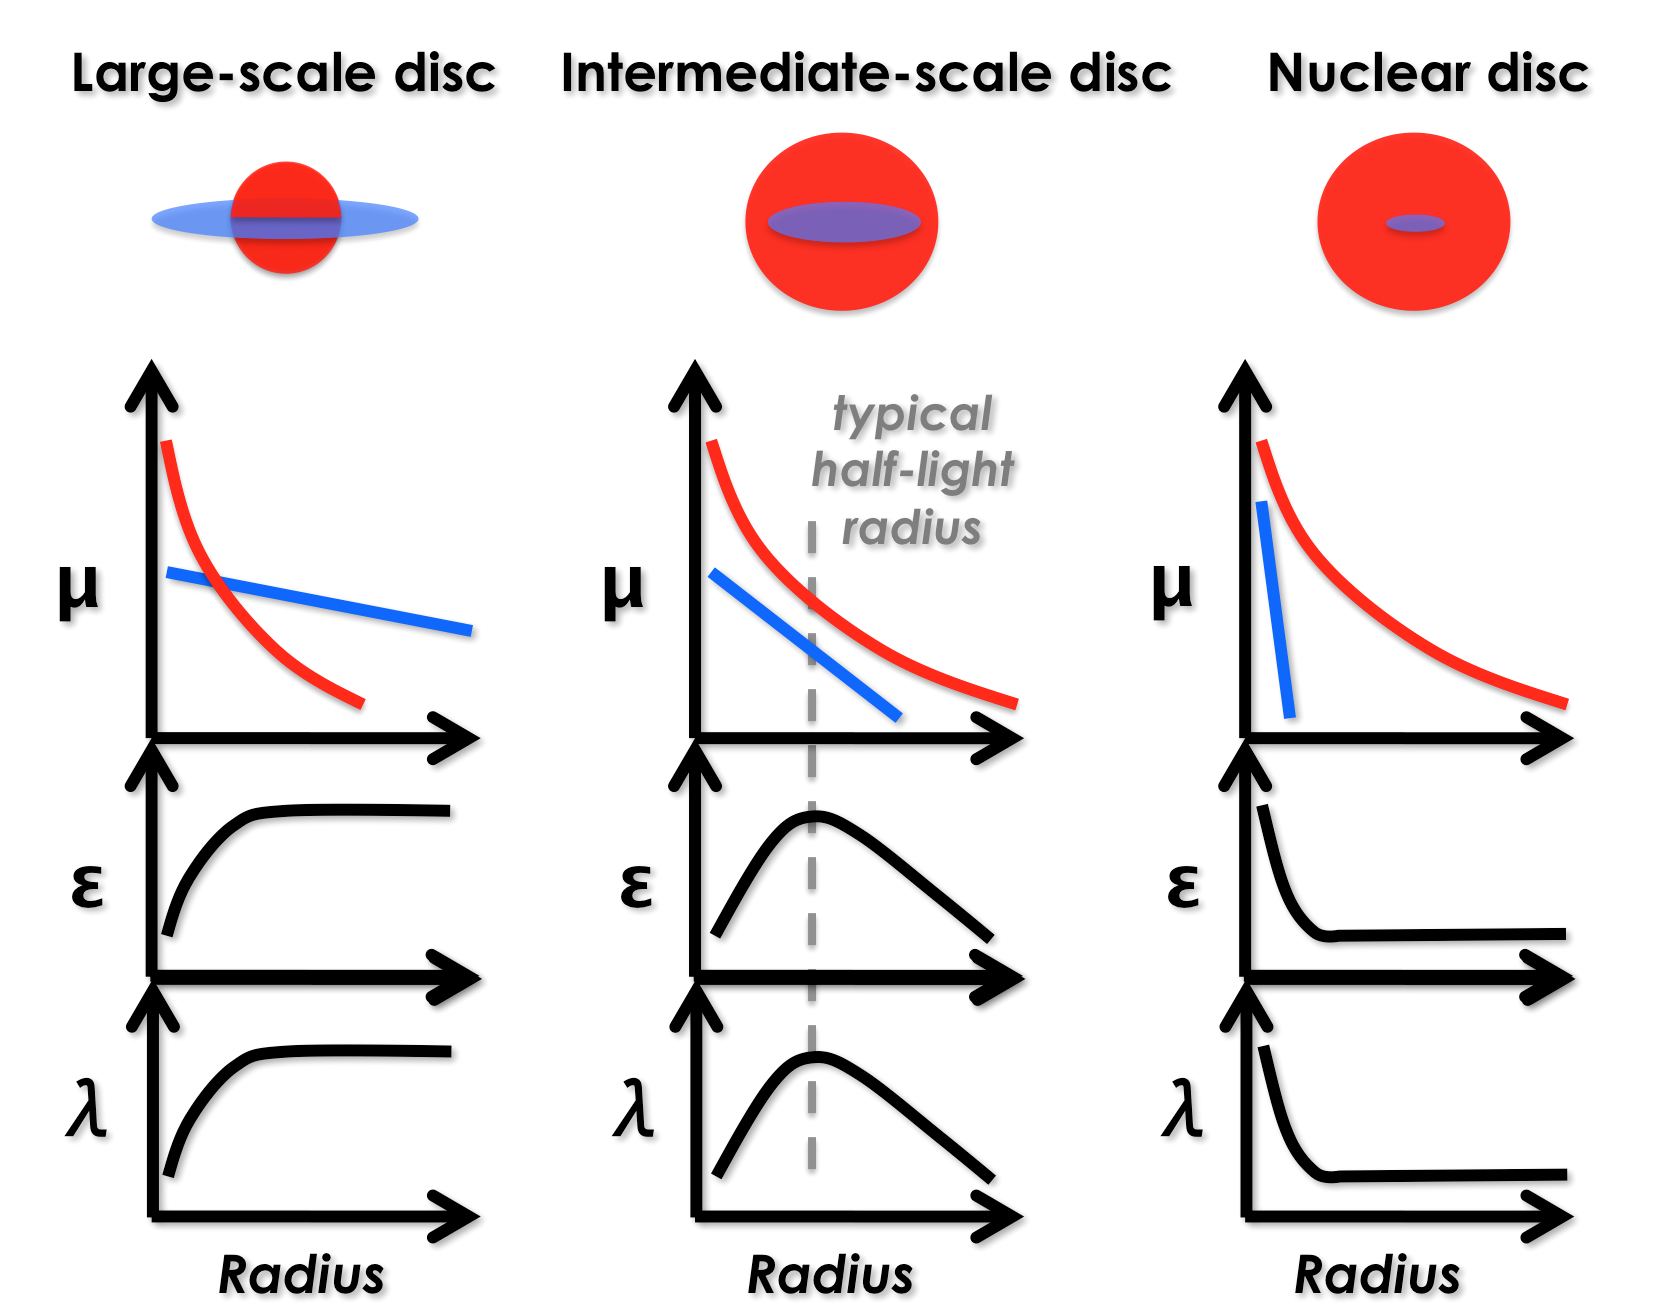
\includegraphics[width=\columnwidth]{images/discmodel.eps}
\caption{Illustration of the spheroid/disc decomposition of the one-dimensional surface brightness profile, $\mu$, 
the ellipticity profile, $\epsilon$, and the specific angular momentum profile, $\lambda$,
for the three prototype early-type galaxy sub-classes. 
In the flux decompositions, the spheroid (or bulge) and the disc are shown with the red and blue color, respectively. 
The left panel shows a lenticular galaxy, composed of a bulge encased in a large-scale disc. 
The right panel displays an elliptical galaxy with (an optional) nuclear stellar disc. 
The middle panel presents an early-type galaxy with an intermediate-sized disc embedded in the spheroid. }
\label{fig:model}
\end{center}
\end{figure}

The awareness that many ``elliptical'' galaxies actually contain embedded stellar discs 
dates back at least three decades 
\citep{capaccioli1987,carter1987,rixwhite1990,bender1990,scorzabender1990,nieto1991,rixwhite1992,scorzabender1995,
donofrio1995,graham1998fornax,scorza1998,scorzavandenbosch1998} and, 
%more recently, intermediate-scale discs were all but unfamiliar to \cite{kormendybender2012} and \cite{krajnovic2013}. 
However, the class of early-type galaxies with intermediate-scale discs has been missed by many galaxy modelers, 
who have labeled as ``unphysical'' \citep{allen2006} those spheroid/disc decompositions in which the disc does not dominate over the spheroid at large radii 
as is observed with spiral galaxies. 
This unspoken bias has led to the rejection of many spheroid/disc decompositions similar to that illustrated in the middle panel of Figure \ref{fig:model}. 
Unsurprisingly, studies affected by this bias have not obtained spheroid/disc decompositions with a spheroid-to-total ratio larger than $0.6 - 0.8$ 
(e.g.~\citealt{gadotti2008,head2014,querejeta2015,mendezabreu2015}). 

The existence of intermediate-scale stellar discs reveals a continuum of disc sizes, 
rather than a dichotomy of nuclear versus large-scale discs. 
The presence of intermediate-scale discs also blurs the distinction between elliptical and lenticular galaxies.
%and creates the need for a new subclass to help bridge the divide. 
The existence of such discs is not only important for our understanding of disc growth in general, 
but accounting for such structure will impact our understanding of galaxy structure, 
with important consequences for galaxy scaling relations. 
%It has recently been argued that the classification scheme for elliptical galaxies should not be their apparent axis ratio as seen on the plane of the sky, 
%but instead their spheroid-to-total ratio, with a continuum from pure elliptical galaxies to disc-dominated lenticular galaxies \citep{graham2014review}.

\section{Galaxies}
\label{sec:xxx}

\section{Implications}
\label{sec:impl}

\subsection{mm diagram}

\subsection{compact massive sph}



%\begin{figure}[h]
%\begin{center}
%\includegraphics[width=\columnwidth]{images/}
%\caption{}
%\label{fig:}
%\end{center}
%\end{figure}


\section{Acknowledgments}
%GS warmly thanks Luca Cortese, Elisabete Lima Da Cunha, Duncan Forbes and Gonzalo Diaz for useful discussion. \\
% referee thank you!!
This research was supported by Australian Research Council funding through grants
DP110103509 and FT110100263.
%This work is based on observations made with the IRAC instrument \citep{fazio2004IRAC} 
%on-board the Spitzer Space Telescope, 
%which is operated by the Jet Propulsion Laboratory, 
%California Institute of Technology under a contract with NASA.
%This research has made use of the GOLDMine database \citep{goldmine} and the NASA/IPAC Extragalactic Database (NED) 
%which is operated by the Jet Propulsion Laboratory, California Institute of Technology, 
%under contract with the National Aeronautics and Space Administration. 

\bibliography{/Users/gsavorgnan/galaxy_vivisection/papers/SMBHbibliography}


\label{lastpage}

\clearpage


\end{document}
